\section{Broadcast Authentication and Device Pairing}


\subsection{Broadcast Authentication: Delayed Key Disclosure} \label{sec:broadcast-auth}

\paragraph{Scenario}
One sender, many unknown (possibly malicious) receivers.
All (legitimate) receivers need to verify the authenticity of the broadcast messages.

\underline{Challenge:}
don't use public key cryptography (computationally expensive, especially on low-power devices), but instead only rely on symmetric cryptography.

\paragraph{One-way hash chain}
Repeated application of a hash function $F$, starting at an original value $s_l$ (see \autoref{fig:hash-chain}).
Due to the one-way property of hash functions an attacker knowing $s_i$ can only compute the subsequent value in the chain ($s_{i-1}$) but not the value $s_{i+1}$ that generated $s_i$.
This allows us to ``use'' the values $s_i$ one-by-one and always reveal a single new value.
See also Merkle hash trees.

\begin{figure}[h]
	\centering
	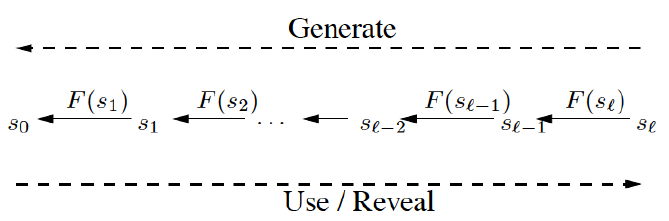
\includegraphics[scale=0.5]{images/8-hash-chain.png}
	\caption{One-way Hash Chain}
	\label{fig:hash-chain}
\end{figure}

\paragraph{Delayed Key Disclosure (TESLA)}
See \autoref{fig:tesla}.
\begin{itemize}
	\item The sender randomly generates a secret $K_l$, computes the entire hash chain and distributes $K_0$ as a ``public key'' to all receivers.
	\item To send a message $M_j$ in the interval $i$, it sends
	$$ P_j = \{ M_j || MAC(K'_i, M_j) || K_{i-d} \} $$
	where $||$ denotes concatenation and usually $d=1$.
	Note that we can send multiple messages in the same time interval using the same key.
	\item To verify a message, the receiver needs to receive $M_j$ and -- at a later time step and in another message -- the key $K_i$.
	They can then compute $K'_j$.\footnote{Why this extra hashing step is needed is ``an implementation detail''.}
	\\
	Then the receivers verify whether the MAC matches and the key $K_i$ does correctly hash down to the pre-loaded $K_0$ and whether the message was received in an interval where the key was valid.
	\item If a key is used after the interval, the message is ignored.
\end{itemize}

\underline{Analysis:}\\
TESLA achieves asymmetry by delaying the explicit disclosure of the self-authenticating keys in cleartext.
It requires time to be loosely synchronised between the sender and receivers.

\begin{figure}
	\centering
	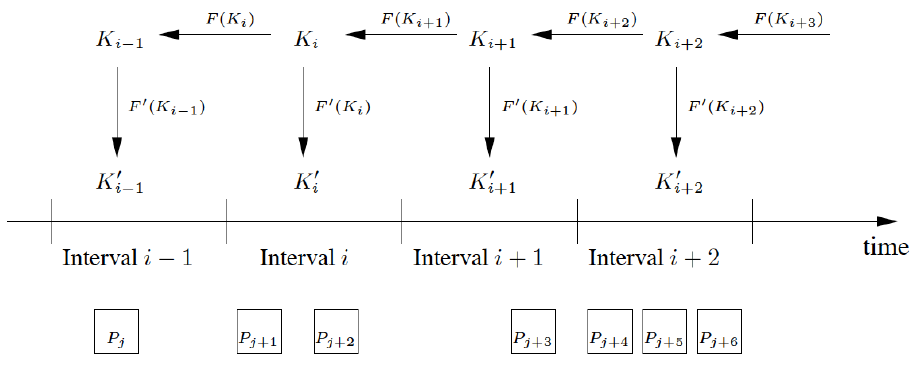
\includegraphics[scale=0.6]{images/8-tesla.png}
	\caption{TESLA}
	\label{fig:tesla}
\end{figure}



\subsection{Device Pairing}

\paragraph{Scenario}
We want to establish a secret key between two wireless devices, in the presence of an adversary.

\paragraph{Diffie-Hellman Key Exchange}
The classic secret key establishment scheme, established a shared key $k_{AB} = g^{ab} \mod p$.
See \autoref{fig:diffie} for a refresher.%
\footnote{We have prime $p$, a generator $g$ of $Z^*_p$ and the Diffie-Hellman assumption stating that the discrete logarithm is hard in some groups.}
However, it is only secure against a passive adversary:
an active attacker can trivially MITM the key exchange.

\underline{Goal:} Authenticate the DH key exchange between two wireless devices, to ensure they have established the same key.

\begin{figure}
	\centering
	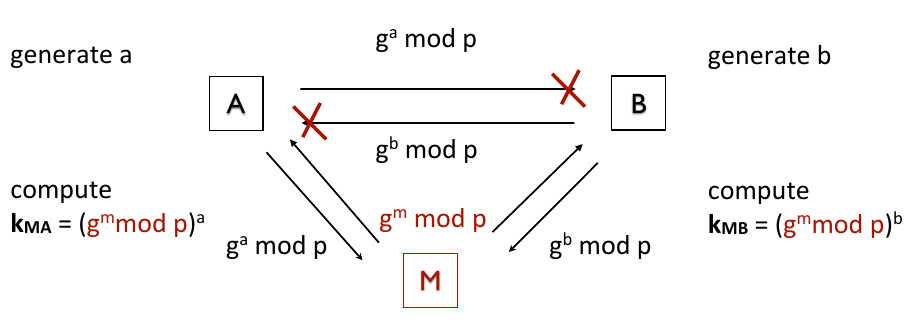
\includegraphics[scale=0.45]{images/8-diffie.png}
	\caption{Diffie-Hellman Key Exchange and MITM Attack}
	\label{fig:diffie}
\end{figure}

\paragraph{Device Pairing Proposals}
A selection:
\begin{itemize}
	\item Short string comparison: hash the key, display the string on both devices.
	\item Seeing is Believing: One device scans a QR code of the other's public key (one-way authentication).
	\item Load and Clear: has public key, map it to a recognisable sentence, read it out loud (text-to-speech TTS).
	\item Integrity Regions: use distance bounding to authenticate the key if the devices are in close proximity.
	\item Resurrecting duckling: first to receive the key becomes the owner for life.
	\item Shake them up: see below.
	\item PIN/Passkey entry: Bluetooth.
\end{itemize}

Note the different security assumptions:
only friends can be close, trust on first use, trusting the human, binding the success of the authentication to the happening and success of authentication (eliminating human error).

\paragraph{Shake them up} \mbox{} \\
\underline{Idea:} \\
Divide time into $N$ slots.
In each slot, randomly either $A$ or $B$ transmit a message.
A message is either 1 (``I am Alice'') or 0 (``I am Bob'').
Depending on who sent the message, this statement is either true or false.
Of course, both Alice and Bob know which is the case.
If the statement is true, set the next bit-to-be-exchanged to 1 otherwise to 0, thus creating a shared secret.
\\
Synchronisation and key exchange are initiated through physically shaking the device (hence the name).

\underline{Analysis:} \\
Assumes that Eve is too far away to distinguish messages from A and B, and can thus not know whether a statement was true or false.
This assumption may NOT hold as it can be attacked using signal fingerprinting to distinguish the source of a signal.
\\
Eve can insert messages, but then A and B will set their bits to different values (since none sent the message and will assume a false statement), thus only creating a DoS situation.

\begin{figure}[h]
	\centering
	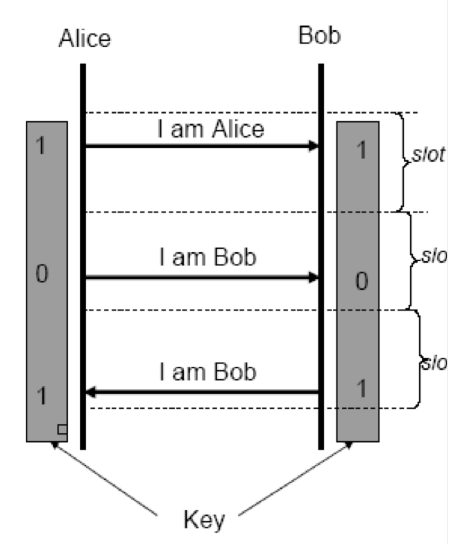
\includegraphics[scale=0.45]{images/8-shake.png}
	\caption{Shake Them Up}
	\label{fig:shake}
\end{figure}

